\newpage
\section{The \acl{SDS}}
This chapter presents the implementation of the newly created design system as a standard for the web user interfaces for SaaS products. \\
Modeling the architecture of a new design system is the first step. Looking at existing design systems and trying to understand how they work and extract requirements in order to develop a common system that fits most products in the SaaS world. \\
Then, this chapter presents the actual implementation of a component, including the technology stack used and the creation process. \\
The chapter concludes with an explanation of the build chain. How the build process bundles all the components and atoms to make them usable for any project. At the end, an example shows the possibilities to integrate the finished bundle into existing software.
\subsection{Architecture}
The actual architecture of the \ac{SDS} describes the structure of the \ac{SDS}. The elaboration models the architecture according to Starke's four-view principle. The four perspectives describe different aspects of the system architecture. \cite{starke_effektive_2020}

\subsubsection{Context perspective}
The context perspective is an overview of the system by modeling out the dependencies to other systems and actors interacting with the system.\\
\begin{figure}[htbp]
    \centerline{
    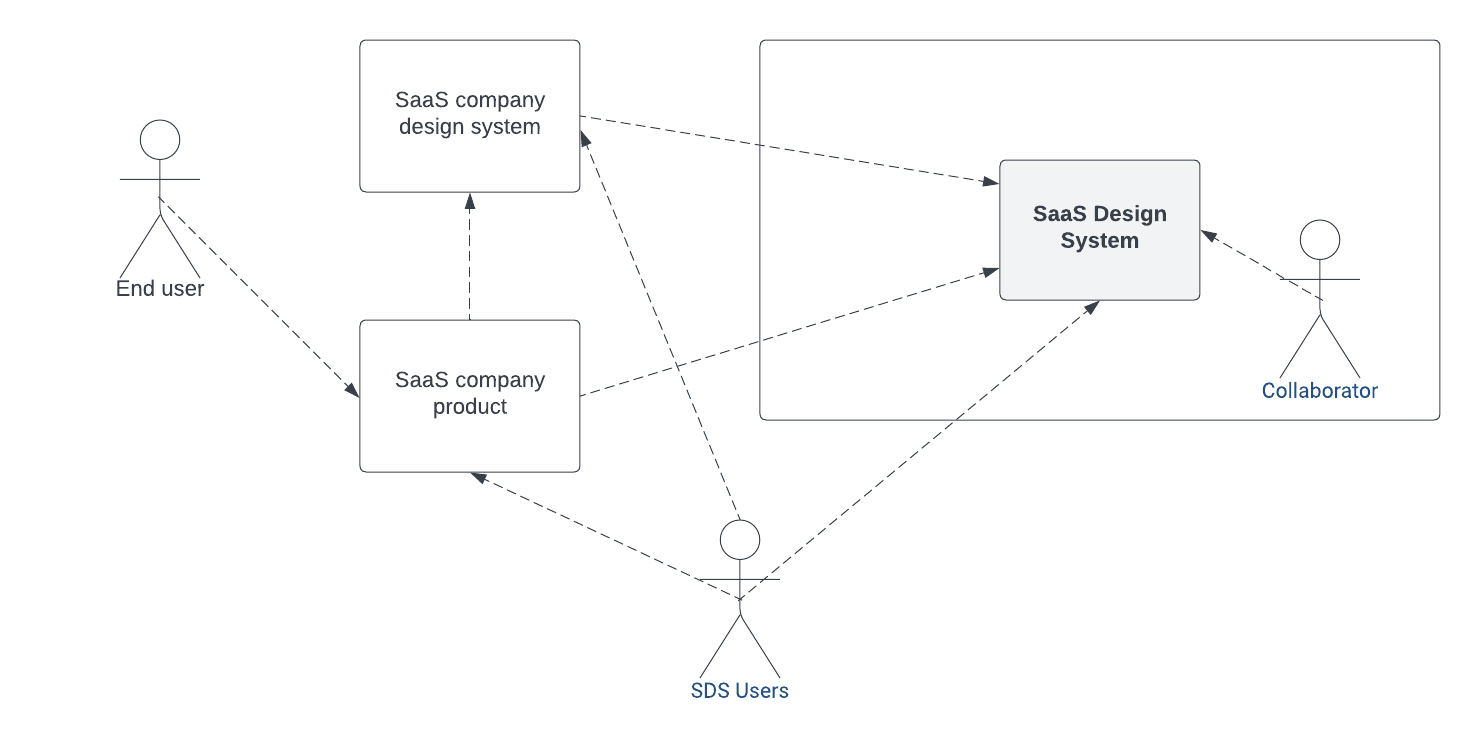
\includegraphics[width=\linewidth]{images/context_view_sds.png}}
\caption{Context perspective of SaaS Design System}
\label{context_view_sds}
\end{figure}

Figure \ref{context_view_sds} shows the first view of \citeauthor{starke_effektive_2020}'s approach to modeling the system architecture - the context perspective. As described in the use case in Section \ref{sds_requirements}, the \ac{SDS} has three stakeholders interacting with the design system. The diagram shows the actively interacting stakeholders (\ac{SDS} users and collaborators) through their connections to the \ac{SDS}. \\
It also shows the "end user" who is not directly connected to the \ac{SDS}, but to a product from a SaaS company. Nevertheless, it is important to mention the end user is the reason why the \ac{SDS} ultimately exists. Following the arrow trail that starts from the SaaS company's product, the \ac{SDS} will always be the one to end up with. This means that the product uses the \ac{SDS} in some way either directly or through the company's design system. \\
The stakeholder who interacts directly with both the SDS and the company's product is the SDS user. User is perhaps a bit misleading, but if you take it that way, this persona uses the SDS to develop or design products from it. This stakeholder may also build the company's design system based on the SDS. This design system is then used by the company's products.\\
The last persona is the collaborator. The collaborator is not interested in applications or design systems that use SDS. The only thing the collaborator wants to do is contribute to the open source project. This is also the reason why this actor is placed inside the system, as the box around him represents the community around SDS.

\subsubsection{Building block view}
The building block view takes the architecture to the next level of detail. The diagrams use the context perspective and go all the way into the presented system, in this case \ac{SDS}. The view lists connections and dependencies to various things like frameworks, databases, components, scripts, and more. \\
The building block view consists of different layers. This makes it possible to focus on important aspects of the architecture in several steps. Diagrams abstract objects so that they can be discussed in more detail later. \cite{starke_effektive_2020} \\

\paragraph{Building block view level 1}
The only gray field in the context view (Figure \ref{context_view_sds}) is the \acl{SDS}. Therefore, the first view shows the top-level architecture of the design system. \\
\begin{figure}[htbp]
    \centerline{
    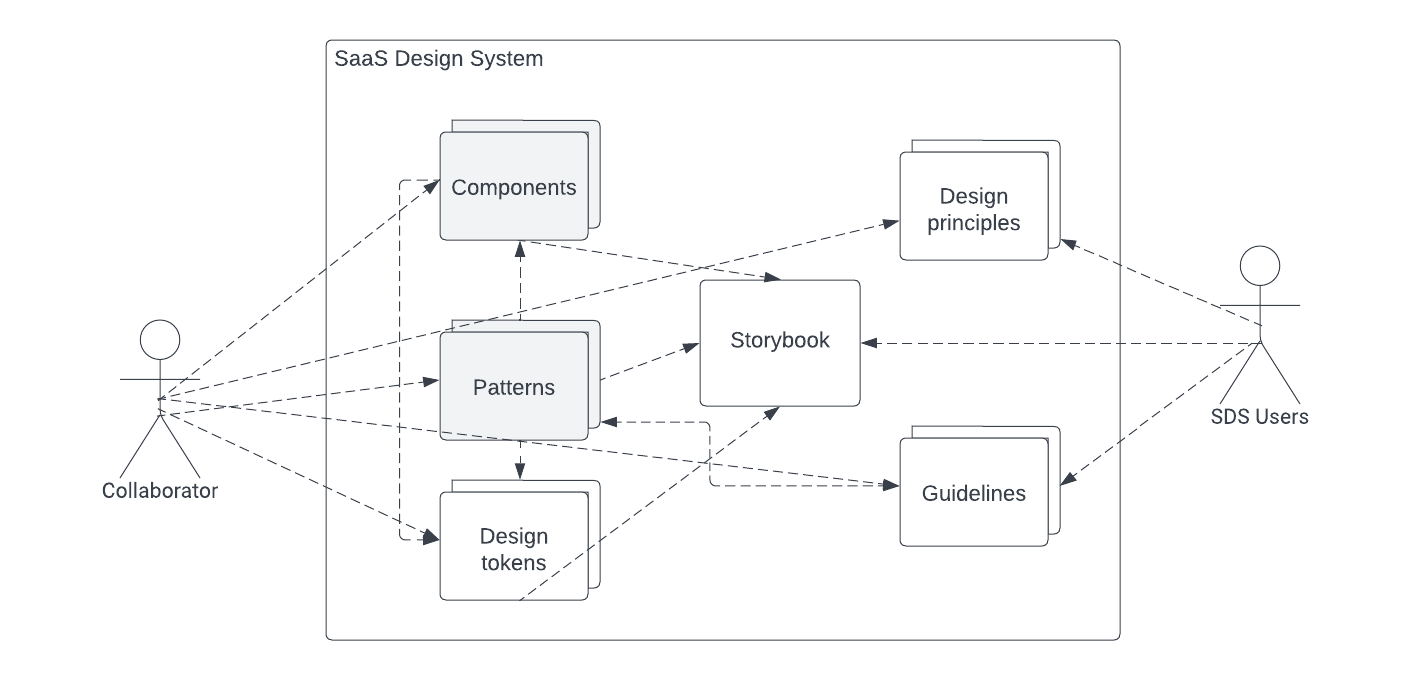
\includegraphics[width=\linewidth]{images/building_block_view_level_1.png}}
\caption{Building block view \ac{SDS} - level 1}
\label{building_block_level_1_sds}
\end{figure}
The level 1 building block view visible in Figure \ref{building_block_level_1_sds} consists of five elements and the two actors interacting with the design system in the context view. Since the SDS is a design system, most of the elements have already been explained in Chapter \ref{design_systems}.\\

\subparagraph{Storybook}
Storybook is the only component that is unknown. Storybook is a tool that helps create and document components on the web. Storybook makes it easy to develop components and document them at the same time. With a variety of plugins written by the community, it offers many possibilities to act as a documentation tool in a design system. \cite{storybook_storybook_nodate}\\
The diagram intentionally shows the building block in the middle. It serves as the central documentation system for components, patterns and design tokens. Therefore, the SDS user interacts with the storybook building block by searching for appropriate components for their use case. The diagram shows other relationships to the programmed assets of the design system. These connections represent the documentation aspect of these building blocks within Storybook.\\

\subparagraph{Design principles}
Design principles are another building block of \ac{SDS}. The diagram in Figure \ref{building_block_level_1_sds} shows that this building block has connections to collaborators and the \ac{SDS} user. This is because both actors use design principles when interacting with the \ac{SDS}. The \ac{SDS} user should keep these principles in mind when creating new applications with the \ac{SDS} or extending the \ac{SDS} to create their own design system. On the other hand, the collaborator keeps the principles in mind when contributing to the system. Components, patterns, and tokens should always follow the design principles. \\
In terms of design principles, the \ac{SDS} strives to keep them lean and easy to understand. This helps the design system to serve as a basis for other design systems. \\
The \textbf{Simple} principle states that component design should not have unnecessary styles or features that make it difficult to extend. This principle underlines the idea of keeping the entire design system lean. Developers understand lean descriptions and clear documentation much better than reading a wall of text. \\
Many products strive to implement accessibility in their products. With the \textbf{Accessible} principle, \ac{SDS} emphasizes the importance of accessible user interfaces. This emphasizes not only significant in terms of inclusion, but also helps accessibility in the overall user experience for all users. Because \textbf{Accessibility} doesn't just come into play when it relates to disabilities, it helps the application with the overall user experience. \\
The third and final principle is \textbf{Solid}. As stated earlier, the \ac{SDS} is a foundation for other design systems to build upon. Therefore, the importance of a stable and consistent API is paramount. Components and patterns should not change regularly. Versioning allows developers to choose their desired version of the \ac{SDS} without having to adapt. For this reason, the design system has deliberately chosen \textbf{Solid} as the third and final principle. \\
The first iteration of the \acl{SDS} principles provides a good foundation on which to build. As described in Chapter \ref{design_principles}, finding the right design principles will take a few iterations to get right. But by starting with \textbf{Simple}, \textbf{Accessible}, and \textbf{Solid}, designers and developers will find the right way to use this design system.

\subparagraph{Guidelines}
The next building block that the SDS user comes into contact with are guidelines. It is obvious that the SDS user needs to know about guidelines in a design system, hence the connection. Furthermore, the diagram shows a bidirectional connection to patterns, which is interpreted as a close cooperation between guidelines and patterns in \ac{SDS}.\\
The design principles just presented form the basis for the \ac{SDS} guidelines. In addition to the core extension, accessibility, and basic use guidelines, some guidelines focus on contributions and collaboration. Therefore, the diagram adds a link to collaborators to the guidelines. This emphasizes that collaborators also consume the guidelines of the design system. As this is an open-source system, as many people as possible should be able to work on it. \\
The extension guidelines address how to integrate \ac{SDS} as the basis for a company's own design system. It shows developers and designers how to create their own from the components provided. The goal of such a guide is to help system developers use the SDS as a foundation. The guide helps developers and designers to build their system on the SDS instead of introducing complex integrations. \\
Since accessibility is also a design principle, a guideline must define what the \ac{SDS} means by accessibility. The guideline should give the user a definition and sources for accessibility. But there should also be a manual for self-designed components to help users implement accessibility. Understanding this guide, users should no longer have accessibility questions when designing new interfaces. \\
As a third guideline, the \ac{SDS} will support the user in using the system. This guide could also be seen as an entry guide and will cover the basics. Importing the design system, proper bootstrapping, and guidance on configuring the system. Such a guideline may seem self-explanatory, but the lack of it often prevents users from using the system. The usage guide should be as simple as possible and cover every small step needed to get started with the \ac{SDS}. \\
One goal of this design system is to be developed by the community for the community. However, this can quickly get out of hand if everyone contributes without guidance. Therefore, it is crucial to introduce some from the beginning. This guide guides how to contribute to the component library and enforce changes to the guidelines and principles. \\
As this design system evolves over time, there should be opportunities to change and adapt. What this will look like in the end will evolve over time. What this will look like in the end will evolve. Some ideas could be a voting process or an RFC process, as is standard in the software industry. \\
Some design systems introduce blogs and forums for knowledge exchange to achieve high interactivity in a design system. In this way, users can connect, discuss and contribute to ideas to further improve the design system. A well-moderated blog and forum will further enhance the community around the \ac{SDS}. \\
Since the \ac{SDS} won't be a product but an open source project, forums and blogs will be the marketing platform to spread the idea of the design system. The goal is to build a strong community around the \ac{SDS}. So that some of the advocates end up contributing to the actual design system. \\
In summary, the guidelines of the \acl{SDS} are about creating a community around the design system. Developer and designers should not only using it for their desired goal, but see the potential to collaborate for the bigger picture behind \ac{SDS}.

\subparagraph{Design tokens}
The last non-gray box in the diagram in Figure \ref{building_block_level_1_sds} is the building block of design tokens. Design tokens form the basis for each component or pattern. Tokens are the smallest unit within the \ac{SDS}. Yet, design tokens have many connections to other building blocks within the design system. 
The connection to collaborators represents their contributions to the design tokens. Collaborators maintain the design tokens. The other two incoming links to components and patterns represent the use of design tokens in them. As well as the link to Storybook described earlier to document Design Tokens for \ac{SDS} users.
\ac{SDS}'s design tokens are not very specific. They consist of basic values like colors, spacing, typography, which were also described in Chapter \ref{layout}.//

Next, it is time to take a closer look at the architecture of the SDS by moving to the second level of the building block view. At the second level, Starke's method performs a more detailed analysis of the building blocks of the components and patterns.

\paragraph{Building block view level 2 - Components}
\begin{figure}[htbp]
    \centerline{
    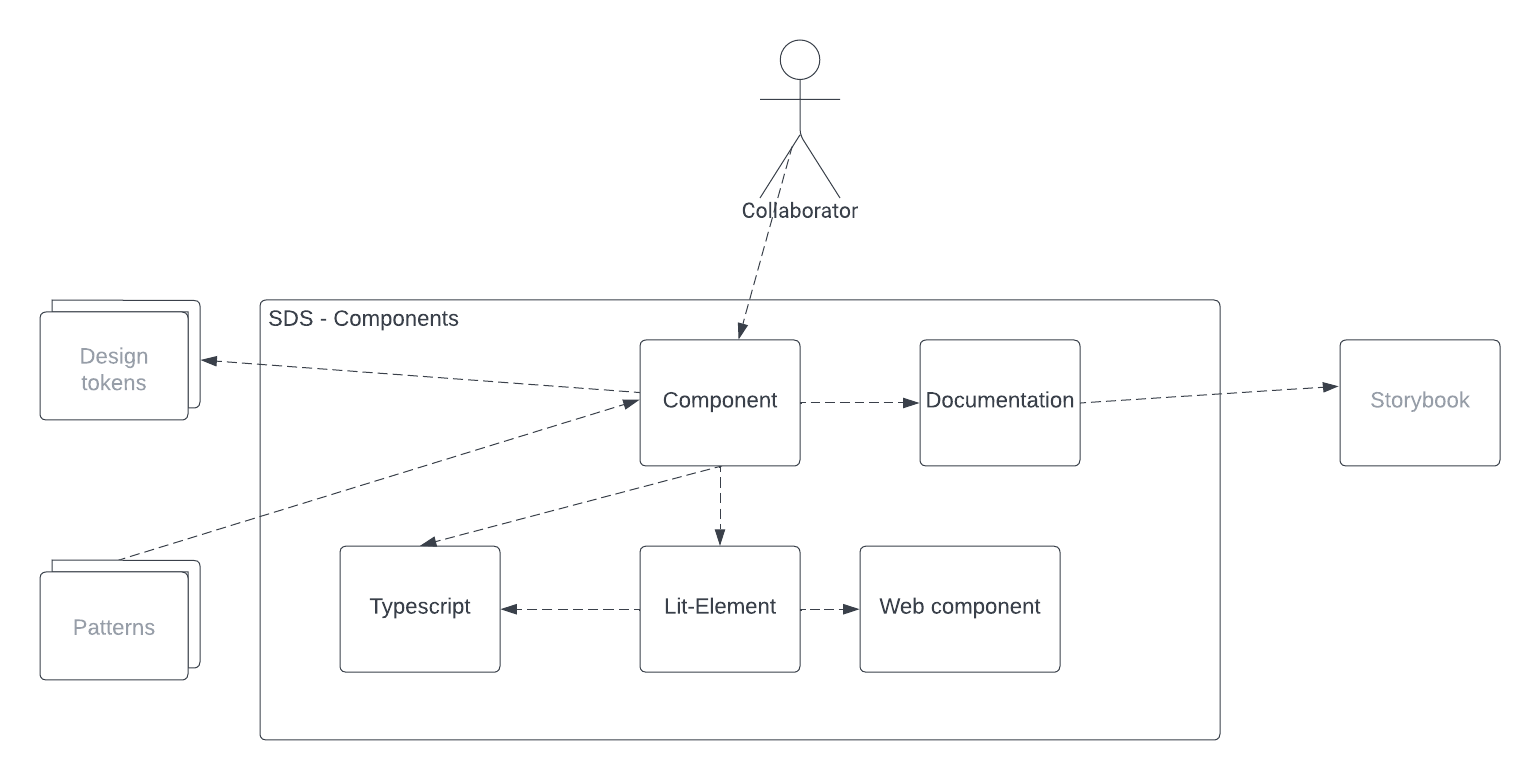
\includegraphics[width=\linewidth]{images/building_block_view_level_2_component.png}}
\caption{Building block level 2 component}
\label{building_block_level_2_component_sds}
\end{figure}
\subparagraph{Components} \label{sds-component}
Without well-assembled components, design systems cannot exist. Therefore, choosing the right technology package for building components is very important. In the case of \ac{SDS}, one of the most essential requirements is that the system is usable independently of the frontend framework used. To achieve this, \ac{SDS} uses the web components supported in almost all modern browsers. As it is possible to create web components without importing libraries or frameworks, it is for \ac{SDS}. \citep{mdn_web_component_nodate} \\

Creating web components natively can be complicated. The Lit Element framework helps developers build web components by eliminating some of the pitfalls of implementing web components from scratch. With a focus on ease of understanding, intelligent DOM updates, and a small package size (5 KB), Lit is a perfect addition for creating components for design systems based on standard web components. \citep{lit_nodate} \\

To further assist developers, \ac{SDS} uses Typescript, a superset of Javascript. It extends Javascript with types and interfaces. Typescript must be compiled into Javascript for the browser to understand, but this allows the developer to find errors much faster because it fails at compile time rather than at runtime. \citep{microsoft_typescript_nodate} \\

The \ac{SDS} uses custom CSS variables to use and provide design tokens for colors or spacing. The design system imports the design tokens into the root element during bootstrapping. In the documentation of the design system exists a page with an overview of all design tokens. \citep{mdn_css_vars_nodate} \\

Last but not least, users must have access to the documentation of the components and tokens. Storybook is the documentation tool for the \ac{SDS}. It has many built-in functions that are useful for documenting components. With MDX, the combination of Markdown templating (MD) and code injection via JSX, it is possible to write fluid documentation without having to jump back and forth between files while documenting components. \citep{otander_markdown_2017} \\

With this technology stack, \ac{SDS} provides users with highly reusable web components that are easy for users to access but also easy for contributors to develop.
\paragraph{Building block view level 2 - Patterns}
\begin{figure}[htbp]
    \centerline{
    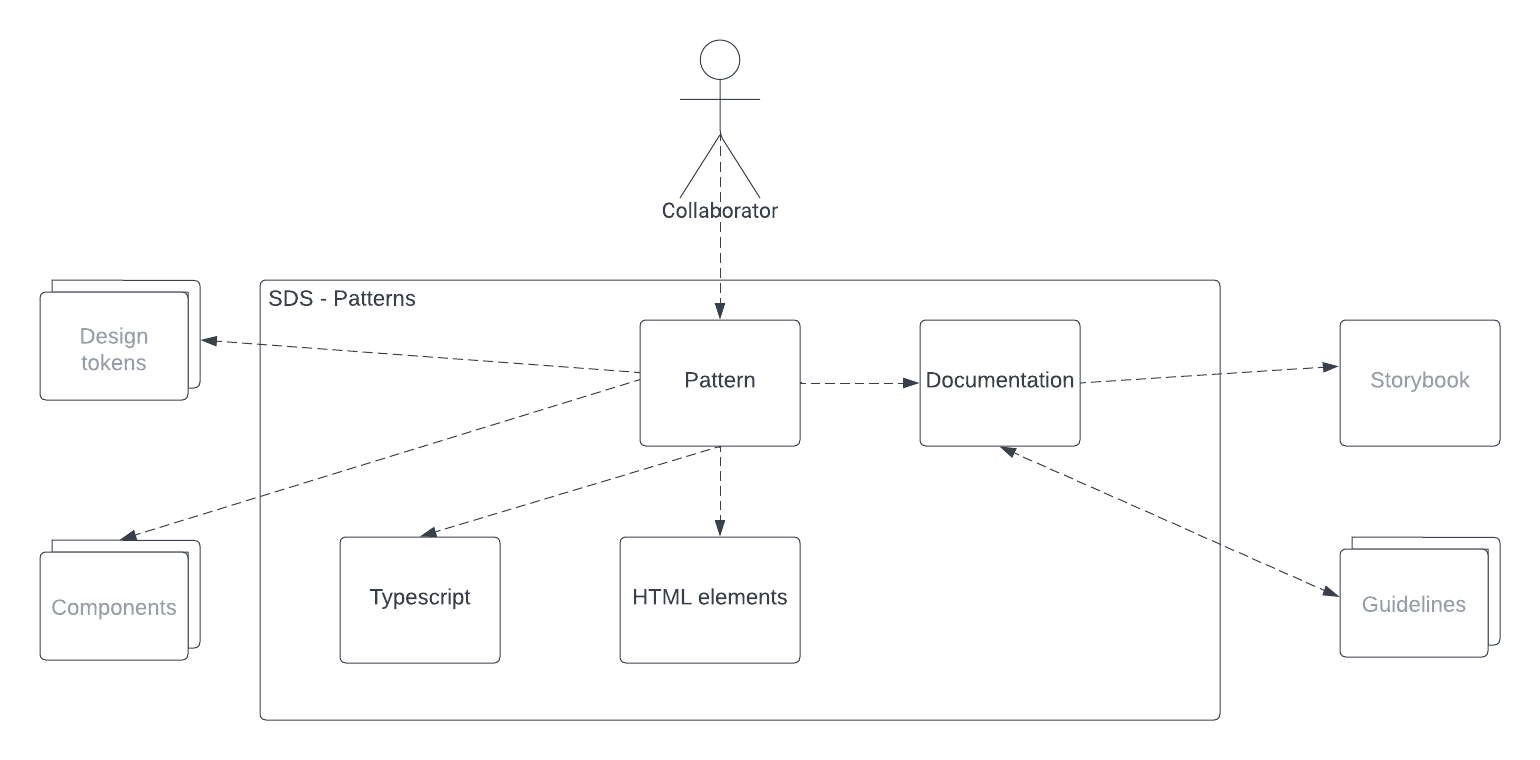
\includegraphics[width=\linewidth]{images/building_block_view_level_2_pattern.png}}
\caption{Building block level 2 pattern}
\label{building_block_level_2_pattern_sds}
\end{figure}



\subparagraph{Patterns}
An essential part of a design systems are patterns. Patterns try to combine the capabilities of a design system with the design of user interfaces. In the case of \ac{SDS}, patterns help developers automatically apply best practices and web standards without having to read an entire text. \\

The combination of standard HTML elements and components from SDS creates patterns in the SDS. These are easily accessible to the developer by copying and pasting code into the desired application that has implemented the SDS. Additional documentation helps the developer to avoid using patterns where they do not belong. \\

SDS patterns come with special documentation that allows for customization and redesign. The documentation enables developers to fulfill their requirements for their own design system.\\

As with the component documentation, live examples show the developer how the design system patterns will work in the final product. Several different examples for each pattern present the possibilities for individual design. \ac{SDS} users have the opportunity to share their creations and application of patterns below the documentation. \\

The big benefit of using SDS is the patterns. They simplify web accessibility compliance and leave enough room for individual user designs. The correct use of patterns is crucial for a successful integration of \ac{SDS} into a product.

\subsubsection{Distribution view}
\subsubsection{Runtime view}

\subsection{Design System Components}\label{sds_button}
An important part of the implementation of a design system are the components. As described in chapter \ref{sds-component}, the components are created using the Lit framework. To see a complete example of a component constructed with design tokens and documented with the storybook, the example of the button component of the \ac{SDS} is presented in this chapter. \\
The components use TypeScript to take advantage of custom decorators. The decorators provided by Lit further simplify the boilerplate code for creating a web component. \\
\lstinputlisting[linerange={1-4},firstnumber=1,caption={Initialization of \ac{SDS} button component},label=ButtonInit]{../Code/src/components/button.component.ts}
In listing \ref{ButtonInit}, the component is initialised with the \texttt{@customElement} decorator by passing the tag name as a string and appending it to an \ac{ES6} class. For it to work properly, the class must extend the Lit Element class. When everything has been implemented as described, the web component is registered and can be used with the defined tag, in this case \texttt{<saas-button>}. \\
In order to see something when the web component just created is used, it must implement the render method. This method expects a \texttt{TemplateResult}. 
\lstinputlisting[linerange={19-26},firstnumber=19,caption={Rendering of \ac{SDS} button component},label=ButtonRender]{../Code/src/components/button.component.ts}
Lit element provides the import of a \texttt{html} string literal that can be used to construct the \texttt{TemplateResult} expected by the render function. With this functionality, Lit provides an efficient way to respond to variable changes and intelligently update the \ac{DOM}. \\
Properties also make use of custom decorators and declare properties on web components by writing \texttt{@property} in front of a class attribute (line 19-20, Listing \ref{ButtonRender}). Thus, Lit Element implements change detection and adds automatic type conversion. For a detailed description of the capabilities of this decorator, see the documentation. Whenever the property value of the created button web component changes, the constructed template string reacts to these changes and updates the displayed template accordingly. \\
Last but not least, the web component must use the defined design tokens. Since these tokens are defined by \ac{CSS} variables, they can simply be consumed as follows: 
\lstinputlisting[linerange={5-20},firstnumber=5,caption={Styles of \ac{SDS} button component},label=ButtonStyles]{../Code/src/components/button.component.ts}
The Lit Element framework implements a static property of the \texttt{styles} to its classes. To make it work properly, a string literal \texttt{css} is used to convert a string into the required \texttt{CSSResult} type. In this way it would be possible to consume design tokens via input properties, but to simply manipulate design tokens in one place, the components of \ac{SDS} will use \ac{CSS} variables. In this way, it is possible to customise certain tokens throughout the design system by adapting these tokens. Each component in the \ac{SDS} will use the defined tokens. Line 7-9 in listing \ref{ButtonStyles} shows an example of the use of design tokens for the button component in the \ac{SDS}. \\
Finally, the button component is displayed in Storybook, the documentation tool for \ac{SDS}. Limited to the time frame of this elaboration, the documentation is kept short. Figure \ref{storybook_button} is an example of what the documentation of \ac{SDS} components may look like. A full version of documentation as in other mature design systems will have to be added in a subsequent development of \ac{SDS}. \\
\begin{figure}[htbp]
    \centerline{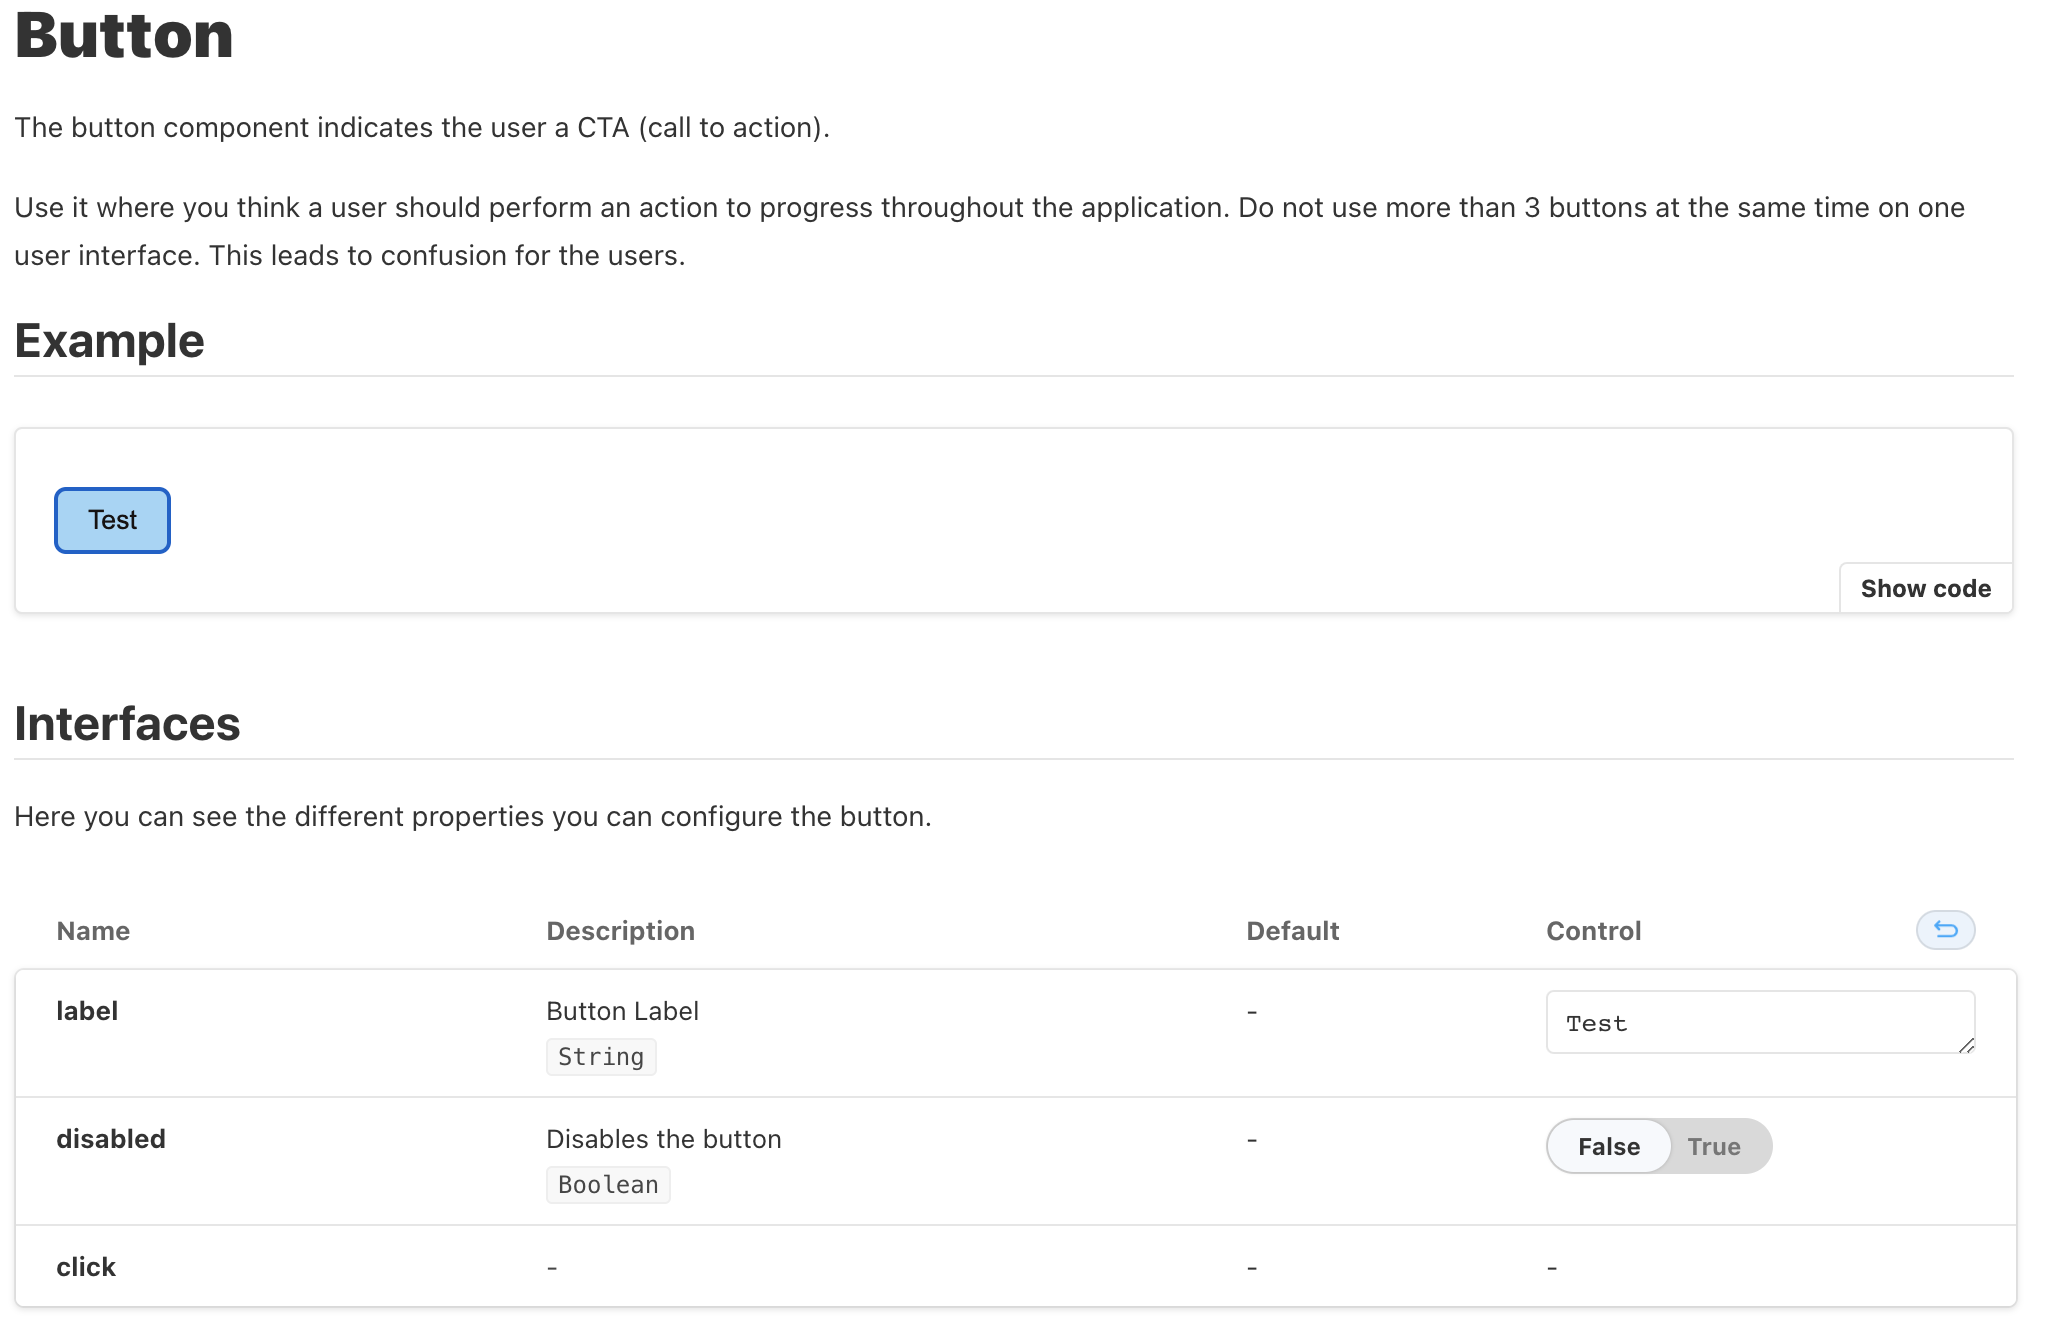
\includegraphics[width=\linewidth]{images/storybook_button.png}}
    \caption{Example documentation of the \ac{SDS} button component}
    \label{storybook_button}
\end{figure}
At the moment, the documentation consists of a short description that briefly explains to the developer how and where he can use the button in his applications. In addition, a live example of the component is presented, which is automatically linked to the properties shown below. When the properties are changed, the example above is updated. This means that the developer or designer who wants to use this component can find out which configuration is most suitable for his use cases. \\
Inspecting the \ac{DOM} element of the button component, the element explorer looks like Figure \ref{button_element_explorer}. When you create a new web component, the saas-button tag is a valid \ac{DOM} element. A new shadow root is opened inside the button component. This allows the web component to isolate styles and elements from the global document. The elements used to display the button component are defined in this shadow root. Also, the styles for the button are defined at the shadow \ac{DOM} level, so the rest of the \ac{DOM} tree never receives these styles. This helps to keep elements and styles separated and easy to understand. \\
\begin{figure}[htbp]
    \centerline{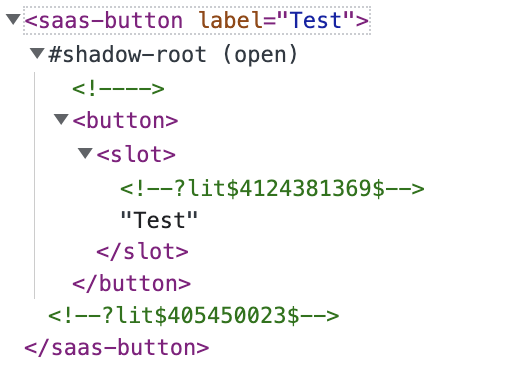
\includegraphics[height=100px]{images/button_element_explorer.png}}
    \caption{Inspection of \ac{SDS} button in elelement explorer}
    \label{button_element_explorer}
\end{figure}
It is important that \ac{CSS} variables declared in the root of the document are also available in the shadow \ac{DOM}. In contrast, style declarations, e.g. for the button element in the overall document, are not applied to \ac{DOM} elements in the shadow \ac{DOM}. \\
The \texttt{<slot>} element in the shadow \ac{DOM} is a default placeholder for anything that is inserted into the \texttt{<saas-button>} element when using the web component. The content is projected within the shadow \ac{DOM} and inserted in place of the \texttt{<slot>} element. This makes it possible to create nested elements with web components which is useful in many different use cases. \\

The example of a simple button component shows how to create and use the components of \ac{SDS}. From here it is trivial to build all the different components needed to create patterns. This is because patterns, as described, are a combination of components that can be reused in applications. The missing piece to using the \ac{SDS} in an application is integration, which is explained in the next chapter.
\subsection{Design System Integration}
The last step to complete the user story of the SDS is to integrate the system into an application. This chapter explains how to package the SDS and load it into a desired application. It is important that the integration is simple so as not to discourage developers from using the design system. \\

The build process is the first part that is important to understand the integration workflow. Webpack is the build tool used by SDS. As shown in Figure 3 in Chapter 1, the components of the design system are built using Typescript, including the Lit framework and using SCSS for styling. Since Typescript and SCSS are not supported by the browser, they must be processed beforehand. Therefore, Webpack comes into play to compile the code. \\
Webpack uses a configuration file, often called webpack.config.js, to describe the steps by which the code is compiled. This file describes rules that tell Webpack what to do with which files that come into the build pipeline. These rules for SDS look like this:\\
\lstinputlisting[linerange={23-41},firstnumber=23,caption={SDS Webpack rules},label=WebpackRules]{../Code/webpack.config.js}
The rules define regular expressions that are used to assign files with their extensions to the corresponding compilers, which are called loaders in the Webpack world. The loaders used here are build-in. But there are also custom ones that can be integrated into a build process. When using loaders, it is sufficient to include the loader string in the use property of a rule object. For example, in line 25-26, Listing \ref{WebpackRules}, the Typescript loader is matched with the regular expression Typescript to process Typescript files. The same pattern is used in line 34-35, Listing \ref{WebpackRules} to match SCSS files with the default style loader that comes with Webpack.